\begin{center}
    \chapter{Datu analīze}
\end{center}

Tā kā no žurnālfailiem ir iegūti dažādi ar GPU izpildi saistītu notikumu
izpildes laiki, kuri starp risinājumiem ir pēc iespējas ielikti ekvivalentās
vietās, tad vienkārši apskatot tekošo kopējo uzkrāto (kumulatīvo) summu,
var vizualizēt katras platformas izpildes laikus pret pietiekami
līdzīgiem atskaites punktiem (skatīt attēlus \ref{img:sha256_100m_not_found_cum},
\ref{img:gol_10k10k_10k_steps_cum}).

\begin{figure}[!ht]
    \centering
    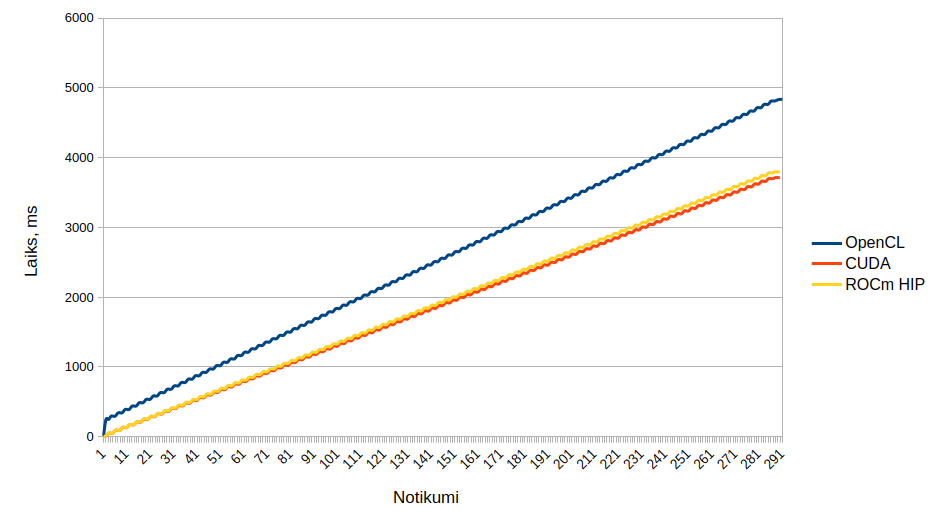
\includegraphics[width=\textwidth]{images/sha256_100m_not_found.png}
    \caption{Paroļu atguvēja izpildes laiki 100m parolēm (parole netika
    atrasta), datu straumes izmērs \( 2^{20} = 1048576\)}
    \label{img:sha256_100m_not_found_cum}
\end{figure}

\begin{figure}[!ht]
    \centering
    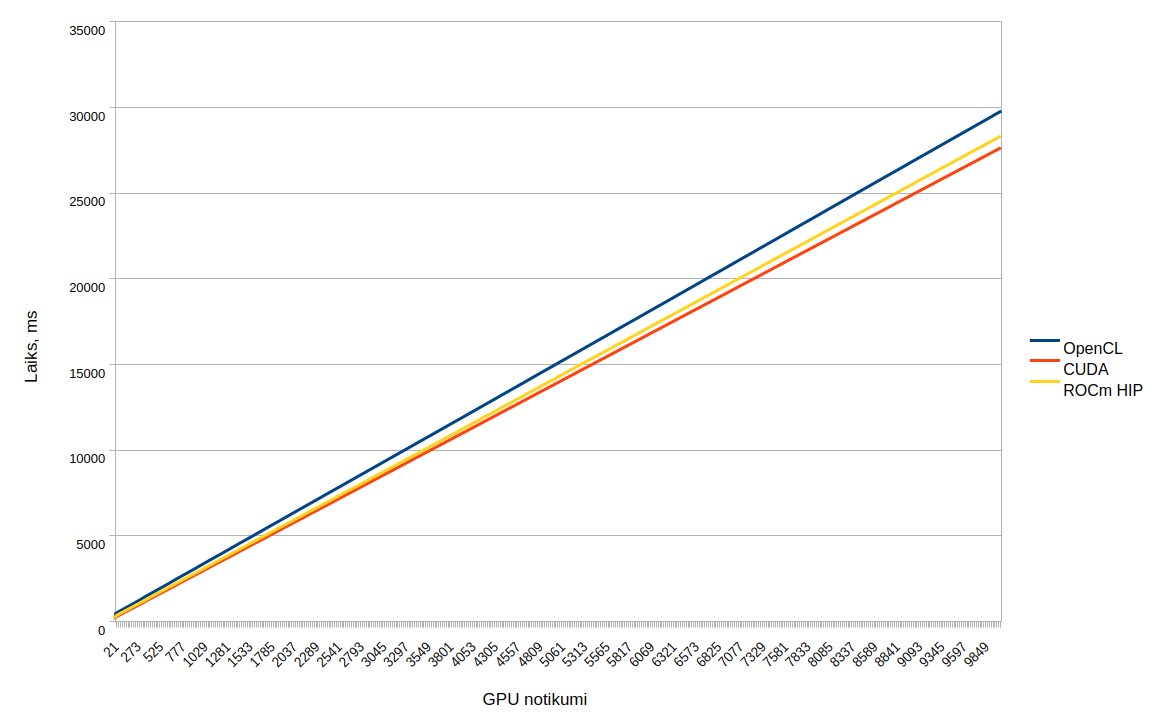
\includegraphics[width=\textwidth]{images/gol_10k_by_10k_10ksteps.png}
    \caption{10000x10000 Dzīves spēle ar 10000 soļiem}
    \label{img:gol_10k10k_10k_steps_cum}
\end{figure}

Pēc grafiem var apstiprināt to, kas jau tika noskaidrots kursa darbā saistībā
ar CUDA un ROCm HIP - ROCm HIP ir neliela virsdarbe, salīdzinot ar
CUDA.\cite{kursa-darbs} Saistībā ar OpenCL platformu, katrs notikums ir,
relatīvi runājot, ar daudz lielāku virsdarbi.

precīzi dati un līknes koef.


buferi salīdzinājums turp un atpakaļ


viena kodola izpilde priekš sha un gol pie dažādiem izmēriem
